\section{Analysis}
\subsection{Homogeneity-measurement of the magnetic field}
To determine the homogeneity of the magnetic field we used a Hall-sensor. As you can see in the diagram below (figure \ref{fig:feld}), a homogeneous field is determined between the two coils which where used to modulate the magnetic field. The error of the depth depends on our accuracy to read the scale attached to the Hall-sensor. 
\begin{floatingfigure}[l]{11cm}
\begin{center}
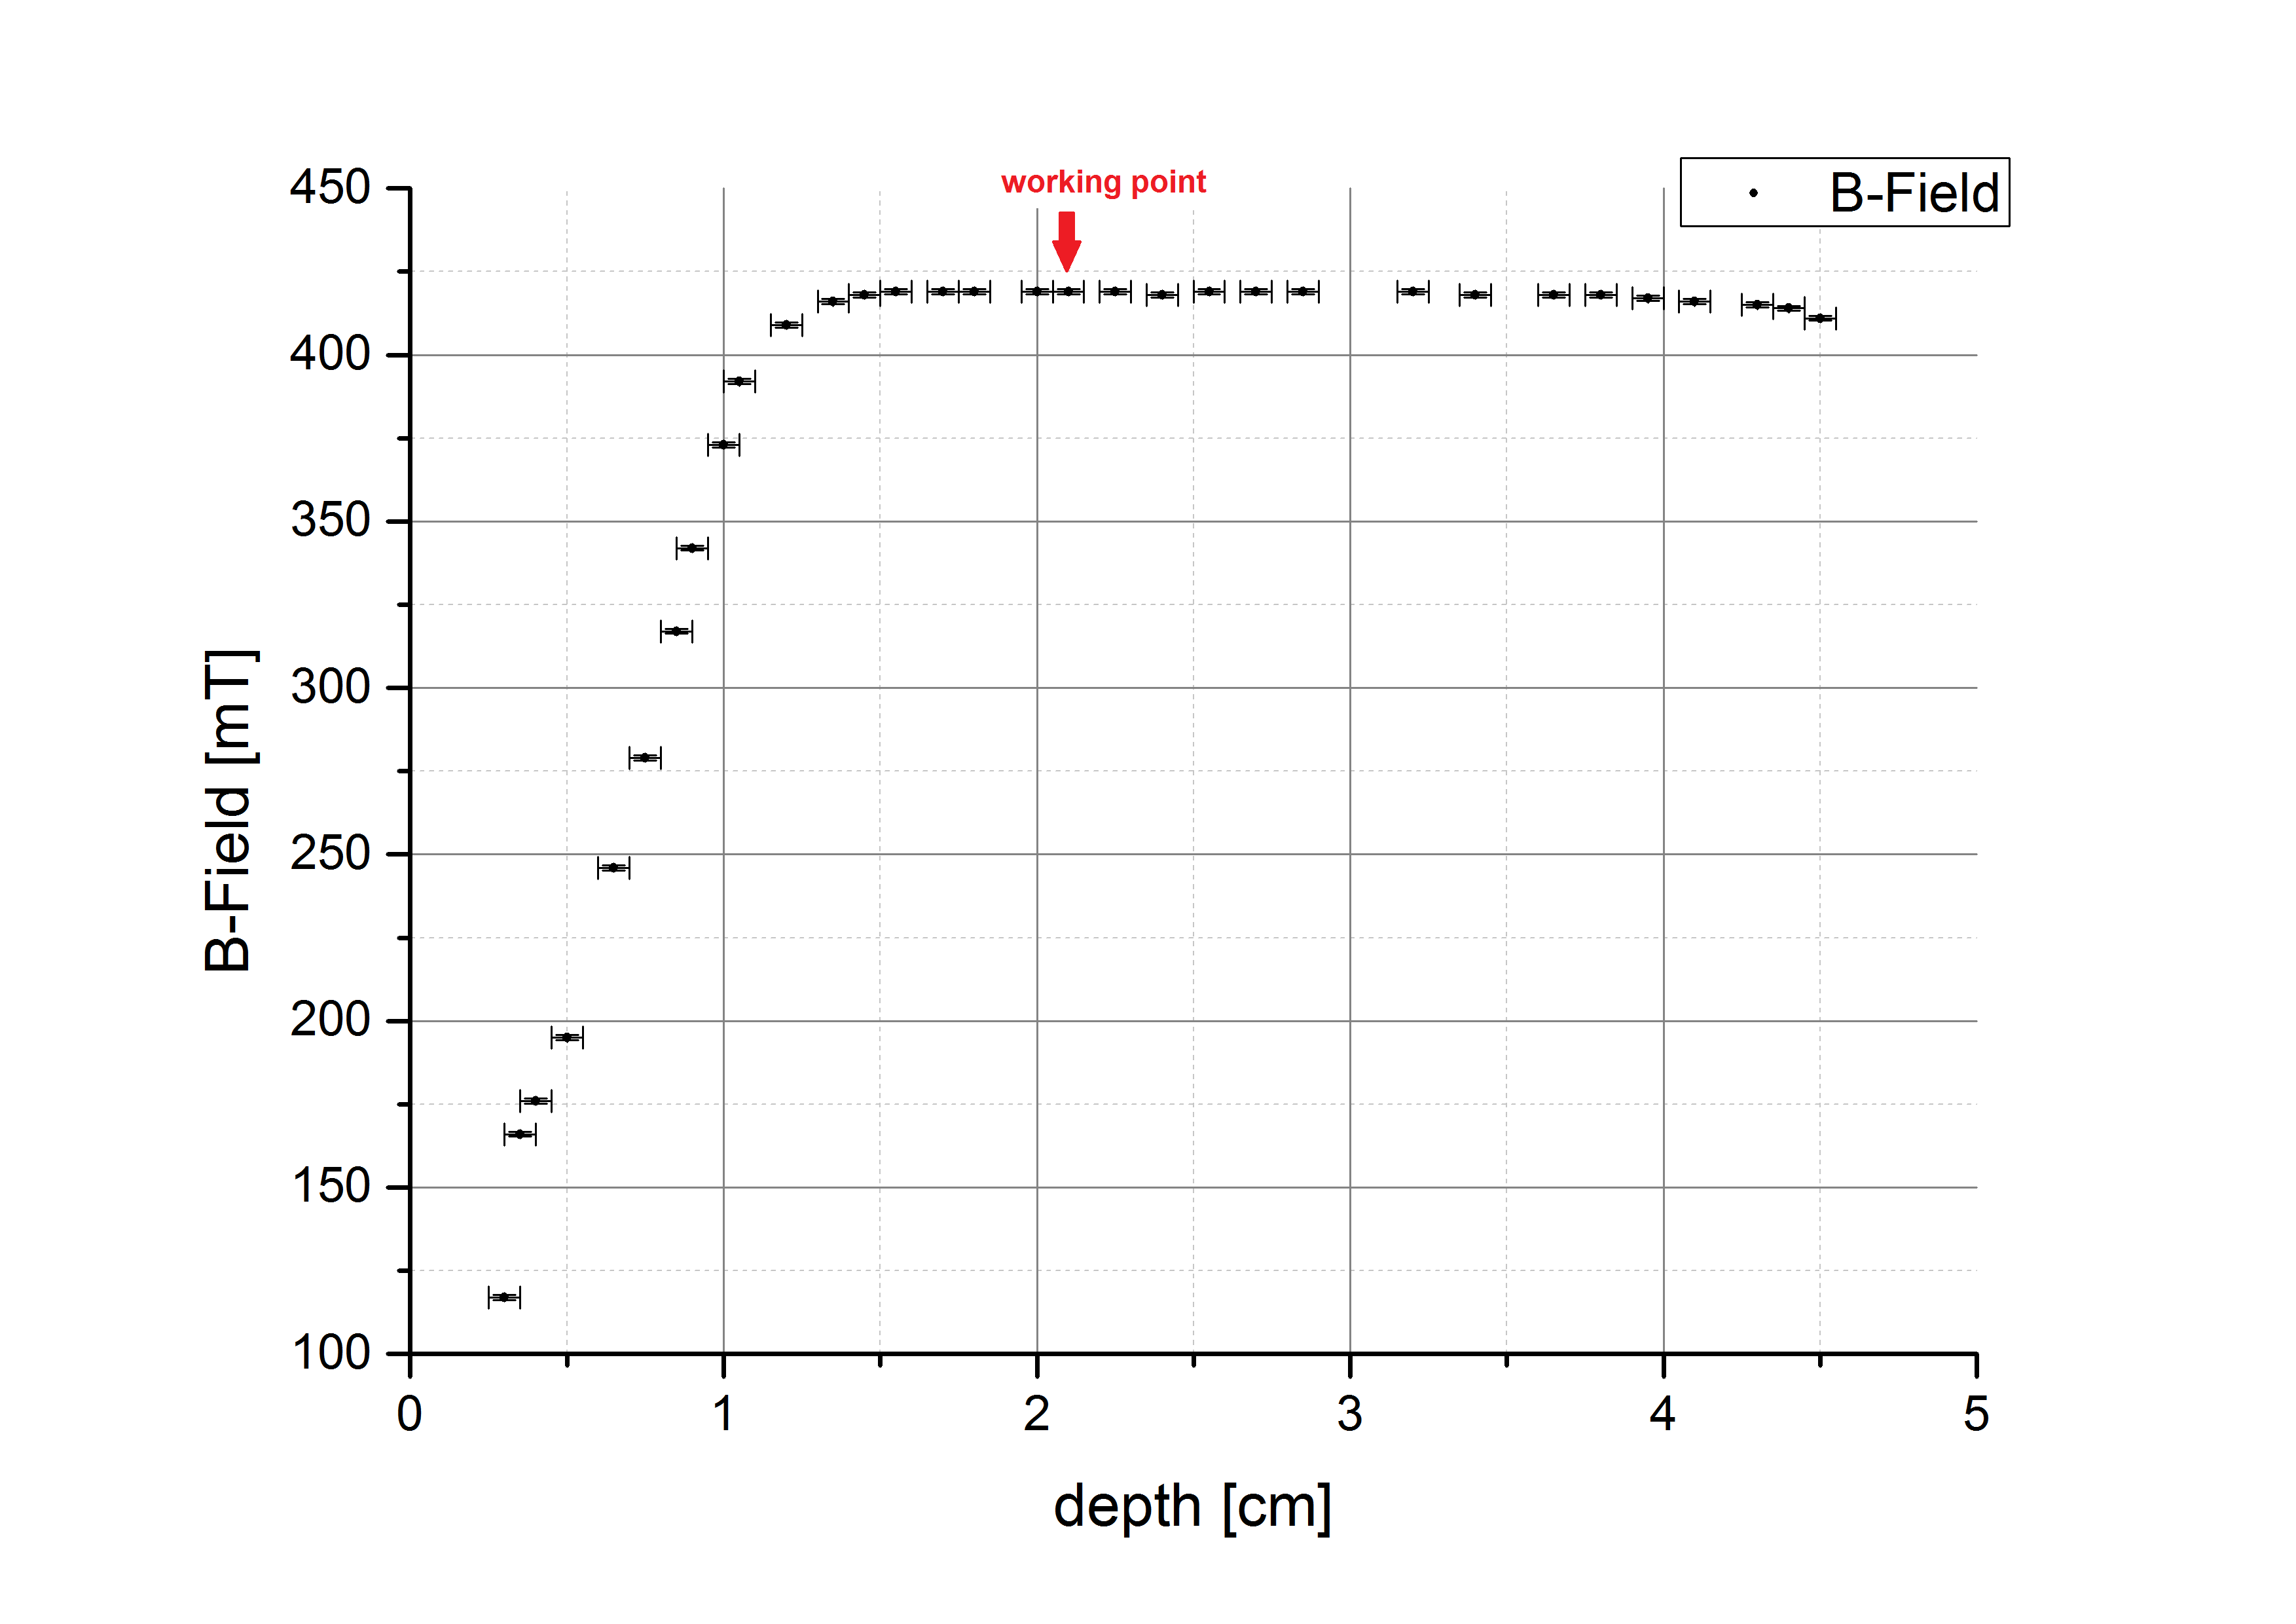
\includegraphics[scale=0.4]{ver_mag_feld}
\caption{Diagram of the homogeneity measurement of the magnetic field}
\label{fig:feld}
\end{center}
\end{floatingfigure}
To determine our error of the B-field we did an extra measurement. The B-field depends on the voltage on the big coils (as can be seen in the realization section above), so we measured the B-field at the same position and the same voltage multiple times by readjusting the voltage again every time. That measurement is shown in the appendix. Out of the statistics of that measurement, we got a standard deviation for the B-field of $s_B=0,8mT$.\\
We decided to use a depth of $d=2,10 cm$ as our working point so we can guarantee that the samples are in the homogeneous magnetic field.\\
~\\

\subsection{Nuclear magnetic moment of $^{19}F$}

\begin{floatingfigure}[r]{8cm}
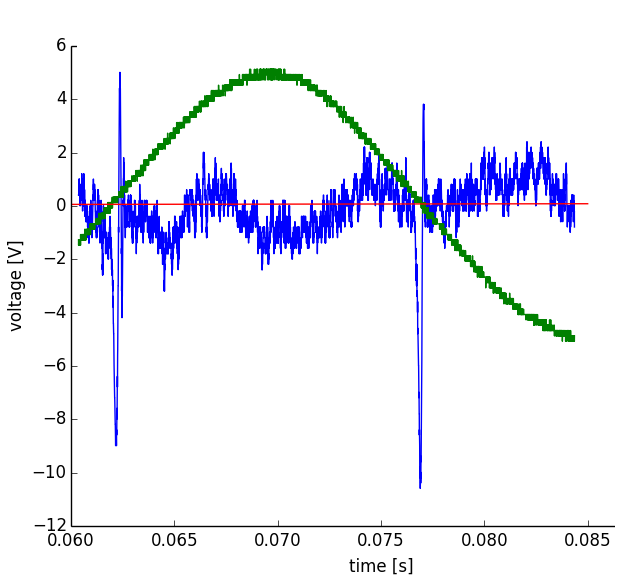
\includegraphics[scale=0.33]{mess_F}
\caption{Signal at our measured resonance frequency with $^{19}F$. To see the peaks in the absorption curve we amplified it by a 100 times.}
\label{fig:mess_F}
\end{floatingfigure}
We measured the resonance frequency as it is described in the 'realization' section. To the given time the signal looked as can be seen in figure \ref{fig:mess_F}. With that settings we measured a frequency for $^{19}F$ of:
\[ \nu_F = 16,61 \pm 0,01 ~ MHz \]
To estimate the uncertainty $s_{\nu_{F}}$ we varied the frequency to see where we can see a difference on the oscilloscope.\\
The nuclear g factor can be calculated by:

\[ \nu = \frac{\gamma B}{2 \pi} ~~~ \Rightarrow ~~~ \gamma = \frac{2 \pi \nu}{B} \]
\clearpage
\[ \frac{g_F \mu_K}{\hbar} = \frac{2 \pi \nu}{b} \]
\[ \Leftrightarrow ~~~ g_F= \frac{h \nu}{\mu_K B}= \frac{4 \pi \nu m_p}{e B} .\]
Its uncertainty can be calculated as follows:
\[ s_{g_{F}}= \sqrt{\left(\frac{\partial g_F}{\partial B} \right)^2 s_B^2 + \left( \frac{\partial g_F}{\partial \nu}  \right)^2 s_{\nu}^2~} \]
So with:\\
$m_p = 1,67262158 \cdot 10^{-27}kg$ as the mass of the photon and\\
$e = 1,602176462 \cdot 10^{-19} C$ as the elementary charge,\\
we get with our magnetic field of $B=419,0 \pm 0,8 ~ mT$ :
\[ g_F = 5,20 \pm 0,01 \]
With that result, we can calculate the magnetic moment of $^{19}F$. By using the formula which is given in the description:
\[ \mu_{K} =\frac{h \nu}{g_{F} B} \]
To calculate the uncertainty of our magnetic moment we use Gaussian propagation:
\[ s_{\mu_{K}}=\sqrt{\left(\frac{\partial \mu_{K}}{\partial B} \right)^2 s_B^2 + \left( \frac{\partial \mu_{K}}{\partial \nu}  \right)^2 s_{\nu}^2~} \]
This leads to a value of:
\[ \Rightarrow \mu_{K}=(5,05 \pm 0,01) \cdot 10^{-27} \frac{J}{T} \]
Our measured value involves the literature value, which is given by
\[ \mu_{K,Lit} =\frac{e\cdot\hbar}{2m_{p}}= 5,05 \cdot 10^{-27} \frac{J}{T} \]
\subsection{Determination of the gyromagnetic ratios}
\subsubsection*{Hydrogen}
For hydrogen, we measured the frequency and its error the same way as described for fluorine. Here we got a resonance frequency of:
\[ \nu_{H} = (17,62 \pm 0,01)MHz \]
We could now calculate the gyromagnetic ratio with that frequency:
\[ \gamma_{1}=\frac{2 \pi \nu_{R}}{B} \]
and the uncertainty using
\[ s_{\gamma_{H}}=\sqrt{\left(\frac{\partial \gamma_{1}}{\partial B} \right)^2 s_B^2 + \left( \frac{\partial \gamma_{H}}{\partial \nu}  \right)^2 s_{\nu}^2~}  \]
\[ \Rightarrow \gamma_{H}=(2,643 \pm 0,005)~\cdot 10^{8}~ s^{-1} \cdot T^{-1} \]
The literature value for hydrogen is $\gamma_{H,Lit} = 2,675 \cdot 10^{8} ~ s^{-1} \cdot T^{-1} $ (source: [NIST]). As one can see our value does not fit the literature value within its limits of accuracy. Further discussion can be found in the part 'Conclusion'.
\subsubsection*{Glycol}
The calculation for the gyromagnetic ratio of glycol is analogue to the calculation for hydrogen. Our resonance frequency here is:
\[ \nu_{glycol} = (17,65 \pm 0,01)MHz \]
So we get a gyromagnetic ratio of:
\[ \gamma_{glycol}=(2,647 \pm 0,005)~\cdot 10^{8} ~ s^{-1} \cdot T^{-1} \]
Again, this does not equal the literature value $\gamma_{Gl,Lit}=2,675\cdot 10^{8} ~ s^{-1} \cdot T^{-1} $. Further discussion can be found in the chapter "Conclusion".